\subsection{Subprocesso de Medição e Análise}

Relembrando que o GQM é uma abordagem top-down orientado a metas para a mensuração de produtos e processos de software,
ou seja, é um processo para definição e interpretação de métricas de software \cite{junior}.

O subprocesso de medição e análise utilizando o método GQM está definido na figura \ref{fig:gqm}

\begin{figure}[h!]
	\centering
  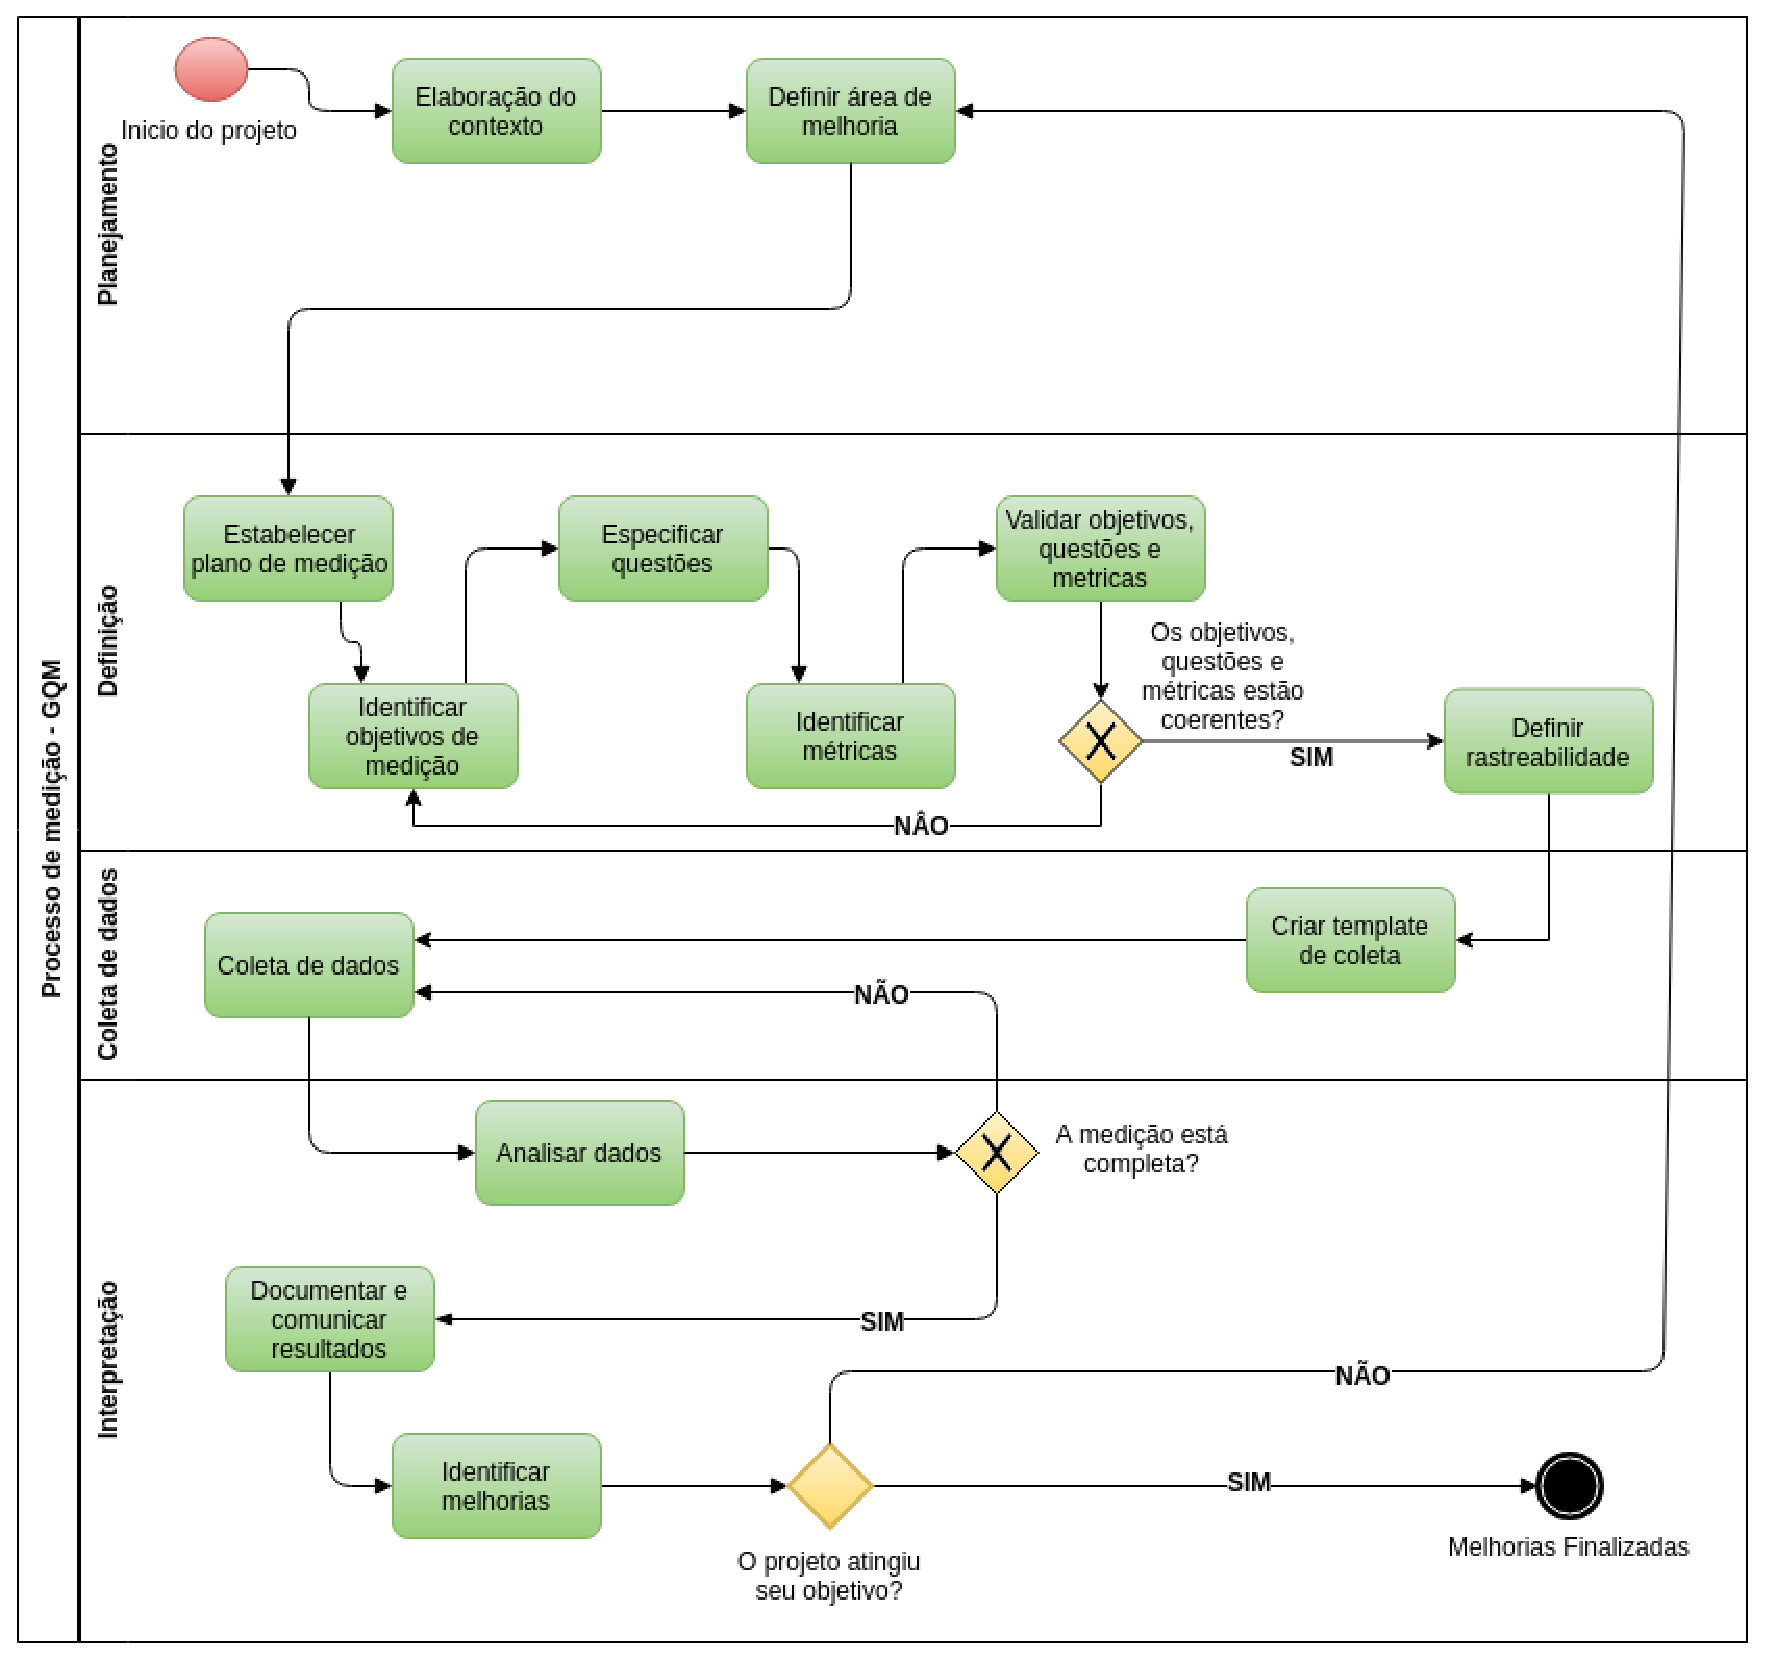
\includegraphics[keepaspectratio=true,scale=0.5]{figuras/processo_gqm.eps}
  \caption[Subprocesso de Medição e Análise (GQM).]{Subprocesso de Medição e Análise (GQM). Fonte: Autor}
	\label{fig:gqm}
\end{figure}

O subprocesso de medição e análise é realizada em paralelo com todo o processo de desenvolvimento, ela se inicia com a identificação do contexto na qual o GQM será aplicado. Com isso será selecionado áreas de melhoria a serem implantadas e assim criado o plano de medição. No plano de medição será definido os objetivos de medição de forma clara e estruturada, será identificado as questões relacionadas aos objetivos propostos e associado às questões será identificado um conjunto de dados de forma a respondê-las quantitativamente.

Duas etapas muito importantes que se segue são a verificação da consistência e completude das métricas em relação ao objeto que desejamos medir e a rastreabilidade das métricas com suas respectivas questões e essas com seus respectivos objetivos de medição.

A coleta dos dados será realizada por sprint. Com os dados coletados, ao final da sprint na revisão e retrospectiva, será analisado o resultado com o resultado esperado no plano de medição. Com isso serão identificados melhorias para as próximas iterações.
